\documentclass[11pt]{article}

% ---------- Packages ----------
\usepackage[margin=1in]{geometry}
\usepackage{amsmath, amssymb}
\usepackage{graphicx}
\usepackage{fancyhdr}
\usepackage{float}
\usepackage{listings}

% ---------- MATLAB Code Listing Style ----------
\lstdefinestyle{matlab}{
    language=Matlab,
    basicstyle=\ttfamily\footnotesize,
    breaklines=true,
    breakatwhitespace=false,
    postbreak=\mbox{$\hookrightarrow$\space},
    columns=fullflexible,
    keepspaces=true,
    frame=none,
    numbers=left,
    numberstyle=\tiny,
    showstringspaces=false
}
\lstset{style=matlab}

% ---------- Paragraph Formatting ----------
\setlength{\parindent}{0pt}
\setlength{\parskip}{0.5em}

% ---------- Header ----------
\pagestyle{fancy}
\fancyhf{}
\lhead{ASEN 5335 Aerospace Environment}
\rhead{Justin Le}
\cfoot{\thepage}

% ---------- Document ----------
\begin{document}

% ---------- Title ----------
\begin{center}
    {\Large \textbf{Homework 4}}\\[0.5em]
    {\large ASEN 5335 Aerospace Environment}\\[0.5em]
    Justin Le\\ 
    \today
    \\[0.5em]
\end{center}

\vspace{1em}
\section*{Problem 1: Field Magnitudes}
\hspace*{2em}Using the WMM model from the NOAA calculator, we find the magnetic 
field in Boulder, CO to be,
\begin{figure}[H]
    \centering
    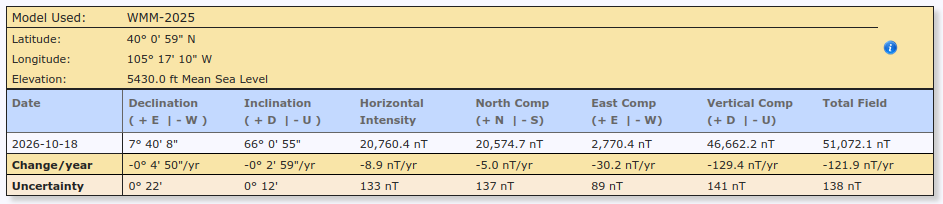
\includegraphics[width=1\textwidth]{Boulder_Magnetic_Field.png}
    \caption{Boulder Magnetic Field}
    \label{fig:Boulder_Magnetic_Field}
\end{figure}

\hspace*{2em}We repeat with the same model for McMurdo Station Anarctica to find,
\begin{figure}[H]
    \centering
    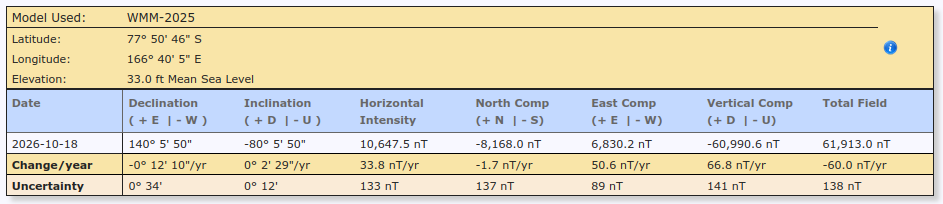
\includegraphics[width=1\textwidth]{McMurdo_Magnetic_Field.png}
    \caption{McMurdo Magnetic Field}
    \label{fig:McMurdo_Magnetic_Field}
\end{figure}

TODO:
\hspace*{2em}Based on the inclination observed at McMurdo, this tells us that... 

\newpage
\section*{Problem 2: Dipole Field}



\newpage
\section*{Problem 3: Magnetopause}



\newpage
\section*{Problem 4: The Ring Current}



\newpage
\section*{Problem 5: Drift due to Gravity}



\newpage
\section*{Problem 6: Geomagnetic Indices}



\newpage
\section*{Problem 7: Geomagnetic Storm}



\newpage
\section*{Problem 8: Key Parameters in the Solar Wind Driving a Magnetic Storm}



\newpage
\section*{Problem 9: The Core}



\newpage
\section*{Problem 10: Magnetospheric Multiscale}


\end{document}
